\section{Overview}
SHRINKS is designed in the way it can operate in two modes: \textbf{stateful} and \textbf{stateless}. Stateful mode is represented by the instance of Unbalanced XMSS (UXMSS) with a root public key \texttt{PK.sf}. An optimized variant of SLH-DSA is used to support the stateless operating mode (which is represented by the public key \texttt{PK.sl}). The root public key is a hashed concatenation of (\texttt{PK.sf}, \texttt{PK.sf}), which is being converted to the Bitcoin address. 

During normal operation with intact state, the user generates signatures according to efficient stateful path. Each leaf of the UXMSS is represented by WOTS+C one time signature instance. UXMSS is right-skewed, which makes the first stateful signature the cheapest from the verification and size perspective (324 bytes) and adds the constant size (16 bytes) and one additional hashing operation for each next stateful signature. 

If the state is corrupted (or the limit for stateful operations is met), the signature can continue operating with stateless mode. Stateless mode utilizes an optimized SLH-DSA variant with WOTS+ signatures in regular XMSS trees on each layer in the hypertree and FORS+C for few-time signature scheme. The general construction of SHRINCS signature is presented on the Figure~1.
\begin{figure}[h!]
    \centering
    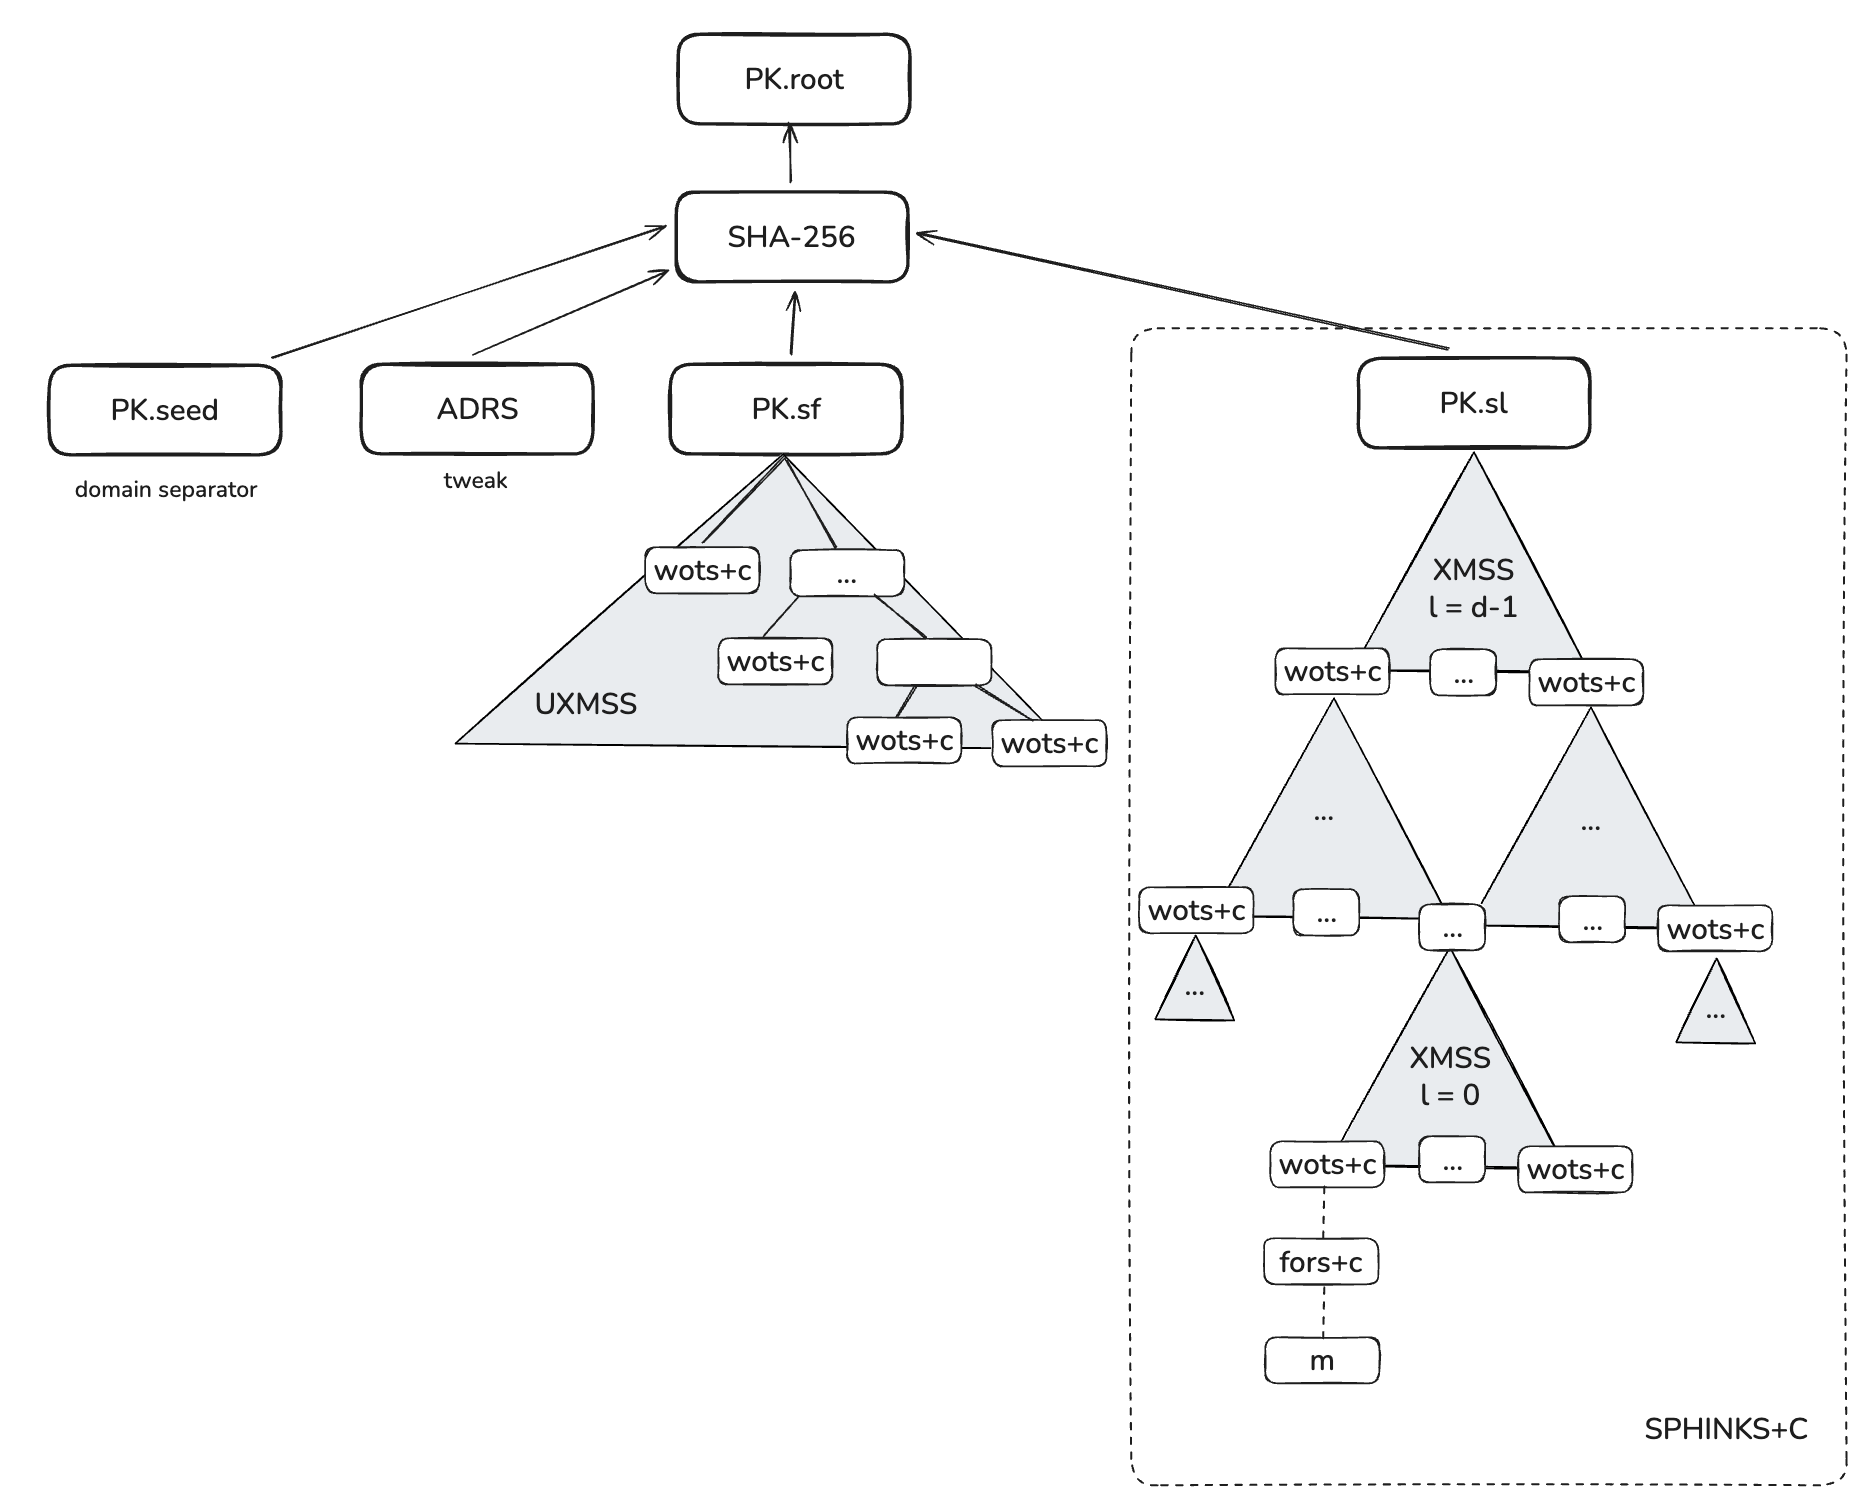
\includegraphics[width=1\linewidth]{content/img/general.png}
    \caption{SHRINCS architecture}
    \label{fig:shrincs}
\end{figure}